\pdfoutput=1
%        File: paper.tex
%     Created: Wed Aug 03 10:00 AM 2011 E
% Last Change: Wed Aug 03 10:00 AM 2011 E
%
\documentclass[12pt]{IEEEtran}
\usepackage{cite, graphicx, subfig, amsmath, wrapfig,hyperref} 
\newcommand{\subparagraph}{}
\usepackage[nobottomtitles*]{titlesec}

%\interdisplaylinepenalty=2500
\hyphenation{}
\title
{Comparison of Global Ionosonde and GPS Electron Density Measurements with the NRL SAMI3 Physics-Based Ionospheric Model during Solar Minimum}
\author{Anish Tondwalkar
\\
{Thomas Jefferson High School for Science and Technology,
Aug 2011, \\ under Carl Siefring, Naval Research Lab, Plasma Physics Division}% <-this % stops a space
\vspace{-1cm}
}
\markboth{SEAP'11 at NRL}{Tondwalkar, A.: Analysis of SAMI2 data}
\begin{document}
\maketitle
%\begin{wrapfigure}{r}{.25\textwidth}
%  \subfloat[The ionosphere. The sun is to the left]{
%  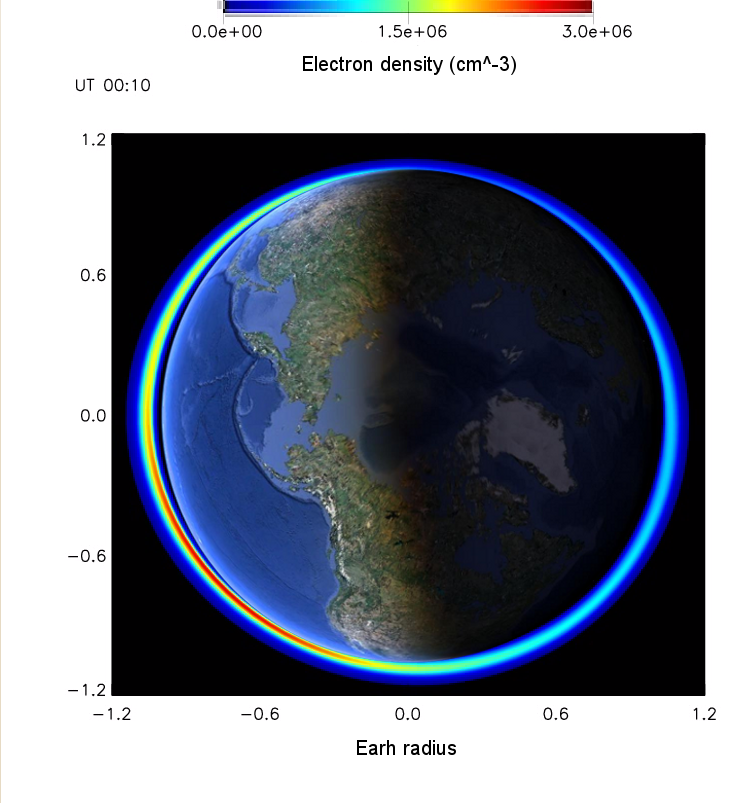
\includegraphics[width=.25\textwidth]{planet}
%  }\\
%  \subfloat[The atmosphere is vertically stratified]{
%  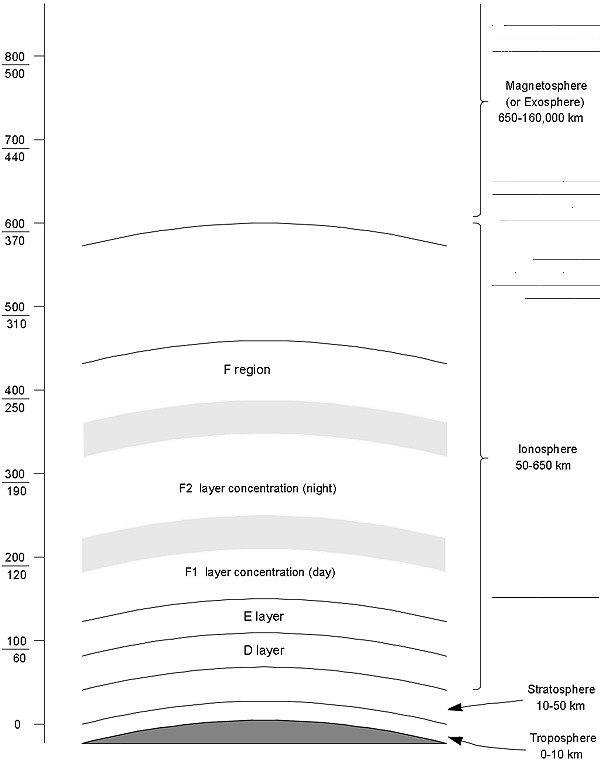
\includegraphics[width=.25\textwidth]{layers}
%  }
%\end{wrapfigure}
\begin{abstract}
  The Naval Research Laboratory is conducting an interdisciplinary physics-based space weather model development and validation program called the Integrated Sun-Earth System for the Operational Environment (ISES-OE). The goal of ISES-OE is to improve our quantitative understanding of the space environment, which can disrupt or degrade operational communications and navigation systems, and ultimately to advance our ability to forecast space weather on multiple time scales.
  
  As part of this program, for validation, numerous runs of the physics-based SAMI3 model have been made and compared to global measurements of electron density.  The data set includes  Ionosonde $f_oF_2$ and $h_mF_2$ measurements and GPS Total Electron Content (TEC) measurements. The comparisons presented will primarily center on Feb. 19 --- April 19, 2008 which contains the most recent Whole Heliospheric Interval (WHI).  This time period, during solar minimum, has only very modest solar activity and is a good test to validate the SAMI3 simulations of the base-state ionosphere. The simulations are driven with a solar irradiance model based on TIMED/SEE measurements and with daily $A_p$ and $f_{10.7}$ indices. Thermospheric conditions are specified with empirical models of the neutral wind (HWM07) and neutral composition and temperature (NRLMSISE-00). We compare SAMI3 with various measurements, including global TEC maps, ionosonde-derived $n_mF_2$ and $h_mF_2$, and GUVI measurements of exospheric temperature.
  
  The results indicate that the SAMI3 has too much plasma in the topside ionosphere and too little in the bottomside ionosphere. Furthermore, SAMI3 shows the $F_2$ peak to be too high and less dense than that of the actual ionosphere. This indicates an overall excessive slab thickness in the model, which was verified in comparison to the data.  It was found that the model consistently had a higher total electron content and slab thickness than the real ionosphere. The electron density of the model was found to be consistently lower than that of the 
actual ionosphere.
\end{abstract}
\begin{IEEEkeywords}
  SAMI, Ionosphere, Modelling, Ionosonde, GPS, Plasma.
\end{IEEEkeywords}
\section{Introduction}
\IEEEPARstart T{he Ionosphere} is a plasma layer of the Earth's Atmosphere that extends upward from about 90km. It is vertically stratified into regions, and it moves up and down again over the course of a day. It is important because the only way to send long distance radio communications is to bounce them off the ionosphere. Waves that are too high in frequency, however, will escape into space. The frequency of the wave that can be sent back down is related to the density by
$$\omega_{pe} = \sqrt\frac{n_e e^2}{m^*\varepsilon_0}$$
Therefore, it is important to know the peak density of the ionosphere at a given time, to know at what frequency we can transmit and expect to get our information back. 
\begin{wrapfigure}{r}{0.25\textwidth}
  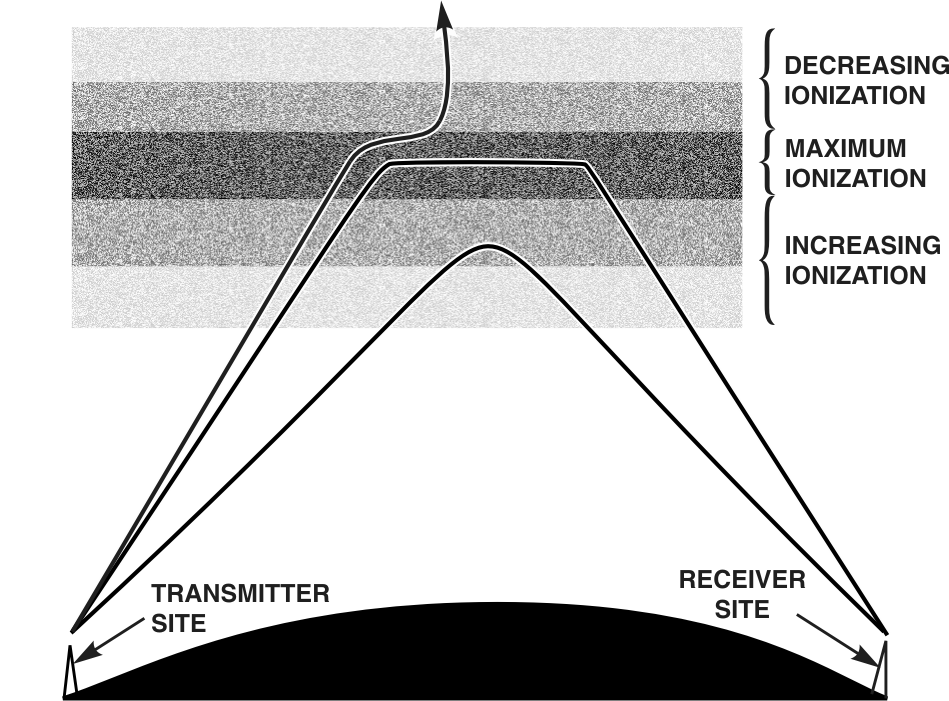
\includegraphics[width=.25\textwidth]{bounce}
  \caption{ Low frequency waves will be sent back from a lower height and frequencies above the maximum transmittable frequency simply go through.  }
  \vspace{1cm}
\end{wrapfigure}

 To first order the atmosphere above about 200 km can be
 described by the pressure/temperature scale heights, as can be seen in Figure \ref{atmos}
 \clearpage 
$$\frac{dP}{dz}=\frac{d \left( nk_BT_n \right)}{dz} = \left< m_n \right> n_ng$$
$$n_n=n_0 e^{-\left( z-z_0 \right)/H_n}$$
$$H_n = \frac{k_BT_n}{\left< m_n \right>g}$$
\begin{figure}[tbp]
  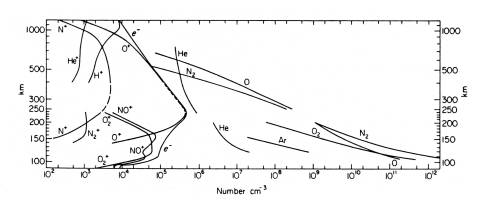
\includegraphics[width=.5\textwidth]{atmos}
  \caption{The ionosphere contains both ions and neutrals. The neutrals fall off with the scale height}
  \label{atmos}
\end{figure}

The ionosphere is ionized by radiation from the sun, and is high up in the atmosphere, and therefore is greatly affected by variation in space weather. Measures of space weather that serve as an input to the model are Solar Extreme Ultraviolet (EUV) flux, $A_p$, and $f_{10.7}$. Here, SAMI3 is coupled with these other models of space weather, and takes inputs from space weather and upper atmospheric models. These models are usually empirical and use simplified physics if any at all to interpolate between measured data points.
The production rate ($P$) due to EUV depends on solar EUV flux ($I$), solar zenith angle ($\chi$) and neutral density ($N_n(z)$).
$$P(\chi,z)\propto I(\chi,z) N_n(z)$$
Note that $P(\chi,z)$ peaks well below the $F_2$ region.
\begin{wrapfigure}{r}{.25\textwidth}
  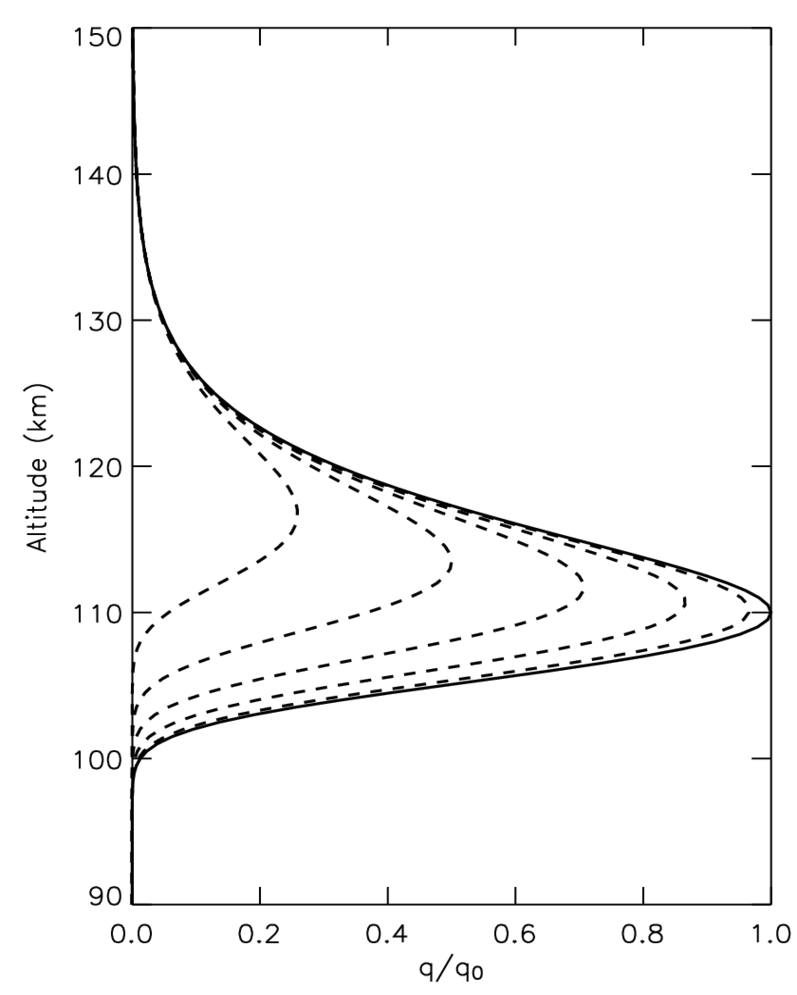
\includegraphics[width=.25\textwidth]{p}
  \caption{Production at various Zenith angles}
  \vskip-.6in
\end{wrapfigure}

  Ionization is lost through recombination and diffusion. 
    The equilibrium electron and ion densities ($N_e(z)$ an $N_i(z)$) are determined by a balance of production and loss.
    Both recombination and diffusion are dependent on the neutral density. The peak density, $n_mF_2$ occurs near the minimum loss condition, where recombination and diffusion are equal.
    \begin{wrapfigure}{r}{.25\textwidth}
      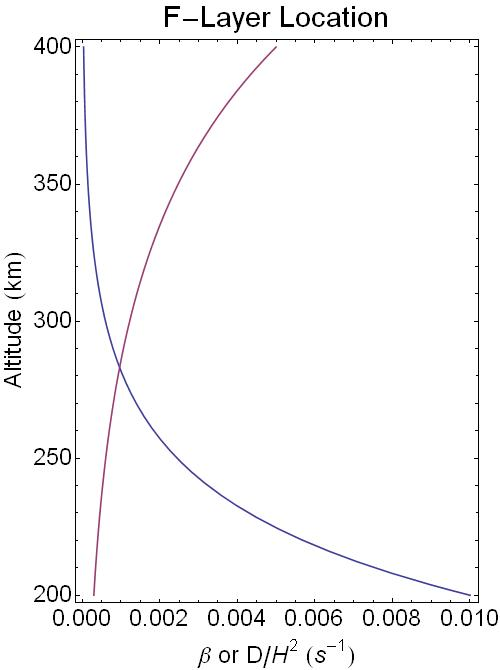
\includegraphics[width=.25\textwidth]{loss}
      \caption{The minimum loss condition occurs when the recombination and diffusion are equal.}
      \vspace{-20pt}
    \end{wrapfigure}

    The ionosphere moves through the course of a day. Figure 6 shows the probability distribution function of ionospheric height at solar maximum in 2002 and at solar minimum in 2008 observed by a large number of ionosondes. Note that both the ionosphere is lower and the composite distribution is bimodal. The yellow distributions represent daytime heights and the blue represent night-time heights. The purple distributions are the composite distributions.

The ionosphere is pushed around by electrodynamic forces and by neutral winds. The $\vec B$-field lines go North-to-South, and the $\vec E$-field lines go East-West.
\begin{figure}[htbp]
  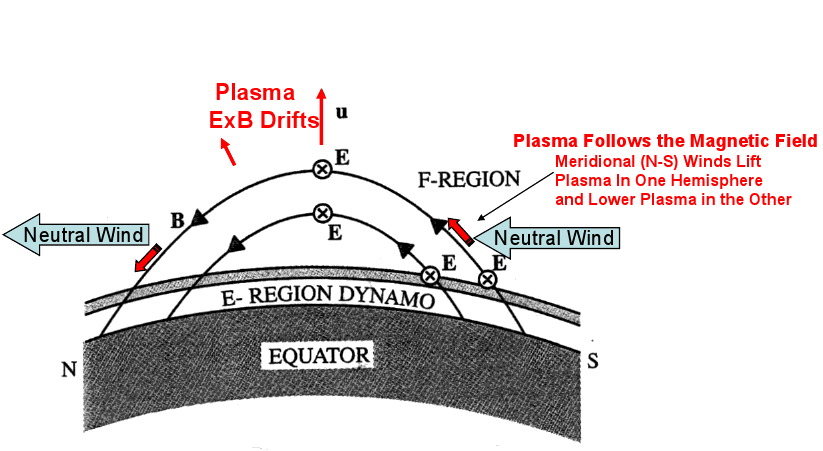
\includegraphics[width=4in]{plasma}
  \caption{Transport: ExB Drifts and Neutral Winds}
\end{figure}
    \begin{figure}[htbp]
     \kern-.2in
      \subfloat[Solar Maximum]{
      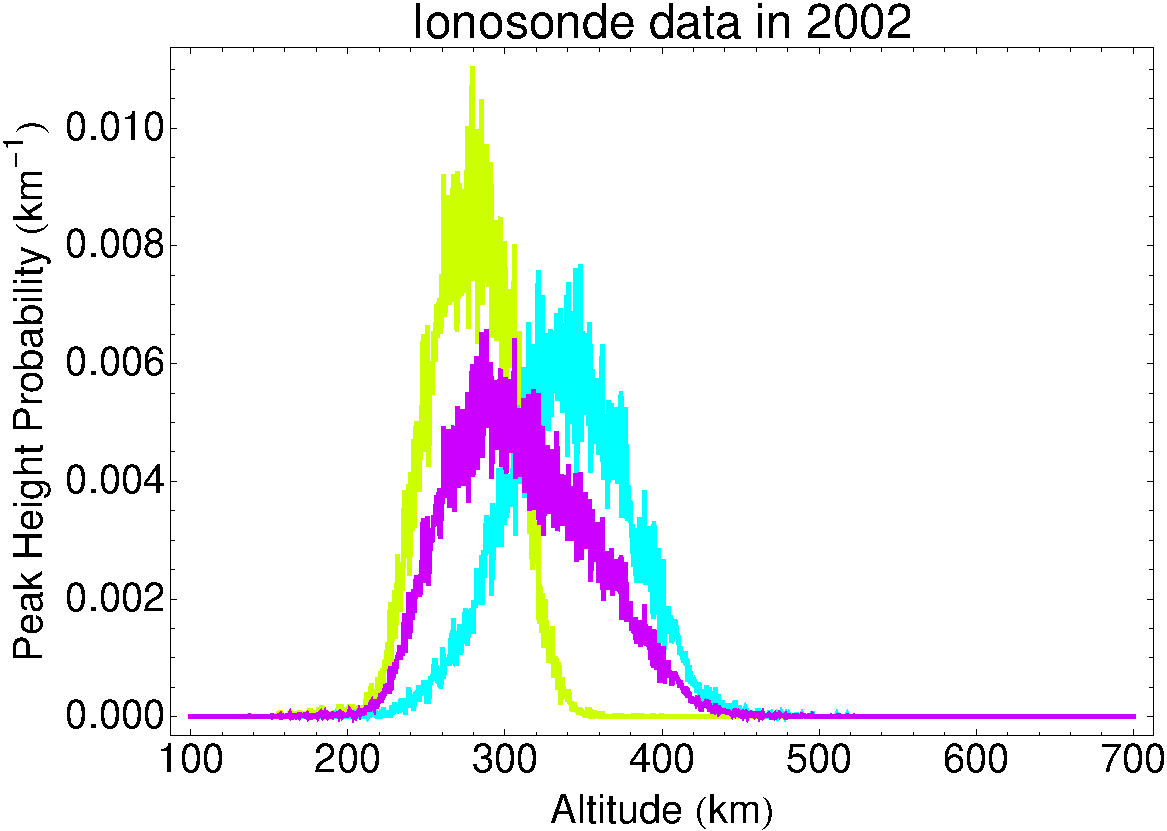
\includegraphics[width=.25\textwidth]{plot}
      }
     \kern-.1in
      \subfloat[Solar Minimum]{
      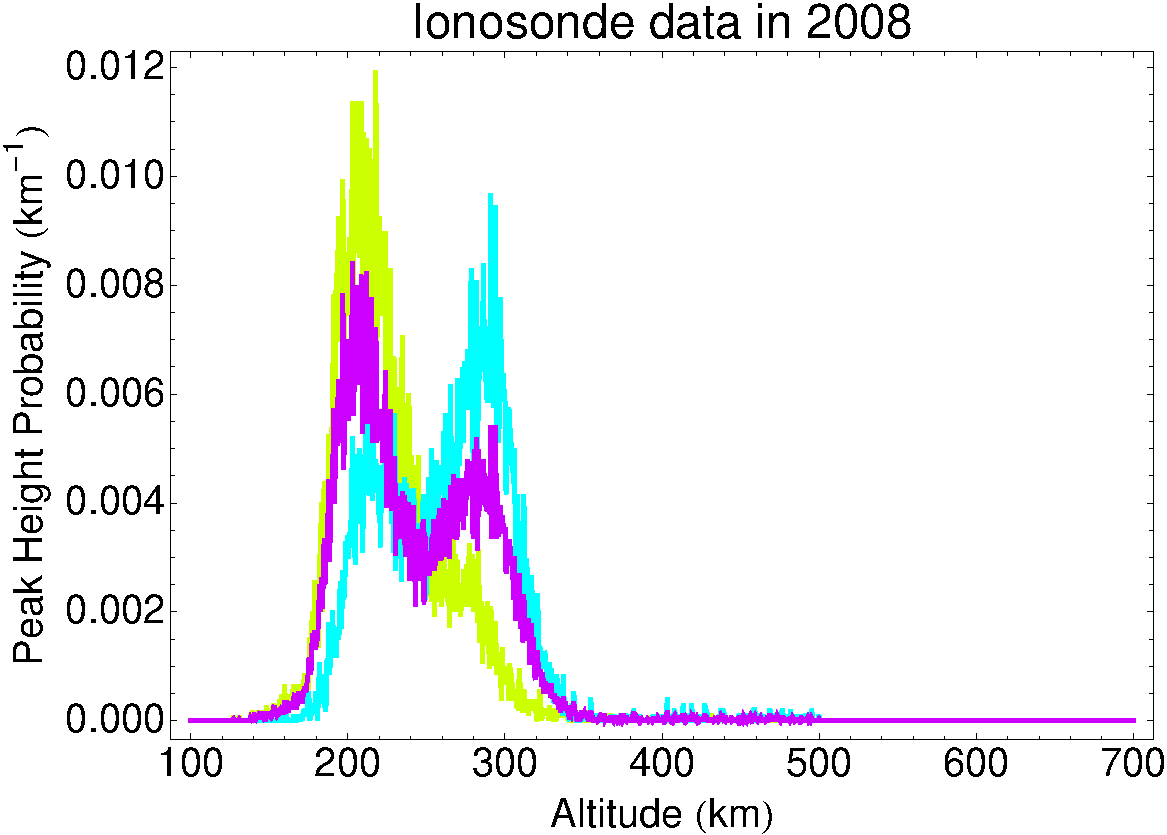
\includegraphics[width=.25\textwidth]{2008}
      }
      \caption{PDF of ionospheric peak height}
      \label{plot}
    \end{figure}
\subsection{SAMI\{2,3\}}
  
{Integrated Sun-Earth System for the Operational Environment (ISES-OE)} is NRL's working group on space weather and its interaction with the ionosphere
    The goal of ISES-OE is to improve our quantitative understanding of the space environment, which can disrupt or degrade operational communications and navigation systems, and ultimately to advance our ability to forecast space weather on multiple time scales.
  
  Feb. 19 --- April 19, 2008 contains the most recent Whole Heliospheric Interval (WHI).  This time period, during solar minimum, has only very modest solar activity and is a good test to validate the SAMI3 simulations of the base-state ionosphere. It has the record lowest density and $f_{10.7}$ out of the recoded solar minima. It was also during the last solar minimum, the lowest point in the eleven year solar cycle.
  \begin{figure}
    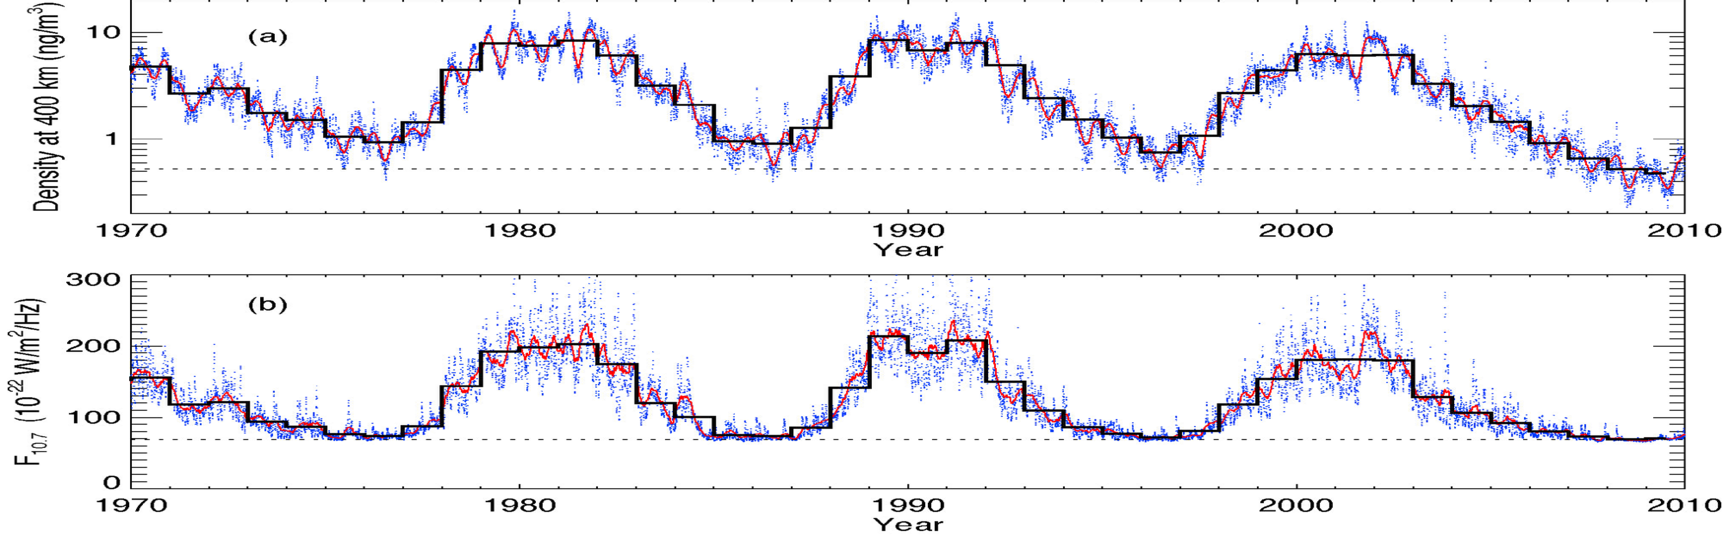
\includegraphics[width=.5\textwidth]{whi}
    \caption{WHI is marked by historically low density and solar flux}
  \end{figure}

  
  SAMI3 is NRL's model of the ionosphere. It is unique in that it solves the momentum equations for electrons and ions, unlike previous physics-based models of the ionosphere:
  \[ \frac{\partial \vec V_i}{\partial t} + \vec V_i \cdot \nabla \vec V_i = 
     -\frac1{\rho_i} \nabla\vec P_i 
     + \frac e{m_i}\vec E + \frac e{m_ic} \vec V_i \times \vec B 
     +\vec g \]
  \[  -\nu_{in} \left( \vec V_i -\vec V_n \right)
     -\sum_j \nu_{ij} \left( \vec V_i -\vec V_j\right) \]
  \[\frac1{n_e m_e} \nabla \vec P_e + \frac e{m_e} \vec E + \frac e{m_ec} \vec V_e \times \vec B = 0 \]
It solves these numerically, along with the temperature equations
  \[\frac{\partial T_i}{\partial t} + \vec V_i \cdot \nabla T_i + \frac23 T_i \nabla \vec V_i 
  +\frac23 \frac1{n_i k} \nabla \vec Q_i =Q_{in} + Q_{ii} +Q{ie} \]
  and the continuity equation for ions, with the production and loss terms added.
  \[ \frac{\partial n_i}{\partial t} + \nabla \cdot \left( n_i\vec V_i \right) = \mathcal P_i - \mathcal L_i n_i \]
  
  MSIS is our model of the neutral atmosphere.  The primary comparison run compensates from MSIS's departure from the actual atmosphere by scaling the outputs from MSIS as they are read into SAMI3. The temperature of the exosphere was scaled by \smash{$0.9607$} the \smash{$[O]$} by \smash{$0.7979$} and all other neutral densities by \smash{$.9697$}. 

\subsection{Measurements}
  \begin{wrapfigure}{r}{.25\textwidth}
    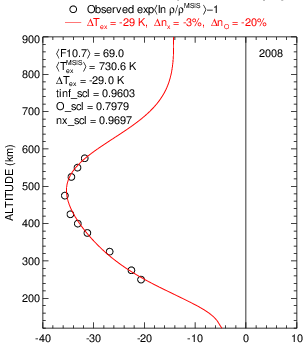
\includegraphics[height=2.5in]{cropped}
    \caption{MSIS atmospheric deviation by percent}
  \end{wrapfigure}

%	{Ionosondes}
Ionosondes profile density vs height.
      The transmitter sweeps all or part of the HF frequency range, transmitting short pulses. These pulses are reflected at heights of $100-400 km$, and the echoes are received by the receiver and analyzed by the control system. The result is displayed in the form of an ionogram, a graph of reflection height (actually time between transmission and reception of pulse) versus carrier frequency.
    
      GPS satellites send out signals, which GPS devices can use to find their location.
    By receiving these signals on the ground at our stations and measuring the phase of the signal form a satellite a known distance away, we can find out the number of electrons it hit on the way here. 
\section{Findings} 

\IEEEPARstart E{ach} plot represents a different station. Note that the frequency/density outputted by SAMI3 are consistently lower than the observed ones. The blue line shows the output from SAMI shifted in both time domain and value to better match the ionosonde data. The shifting is done using a cross-correlation of the data and shows a phase shift of less than two hours in some places. 
    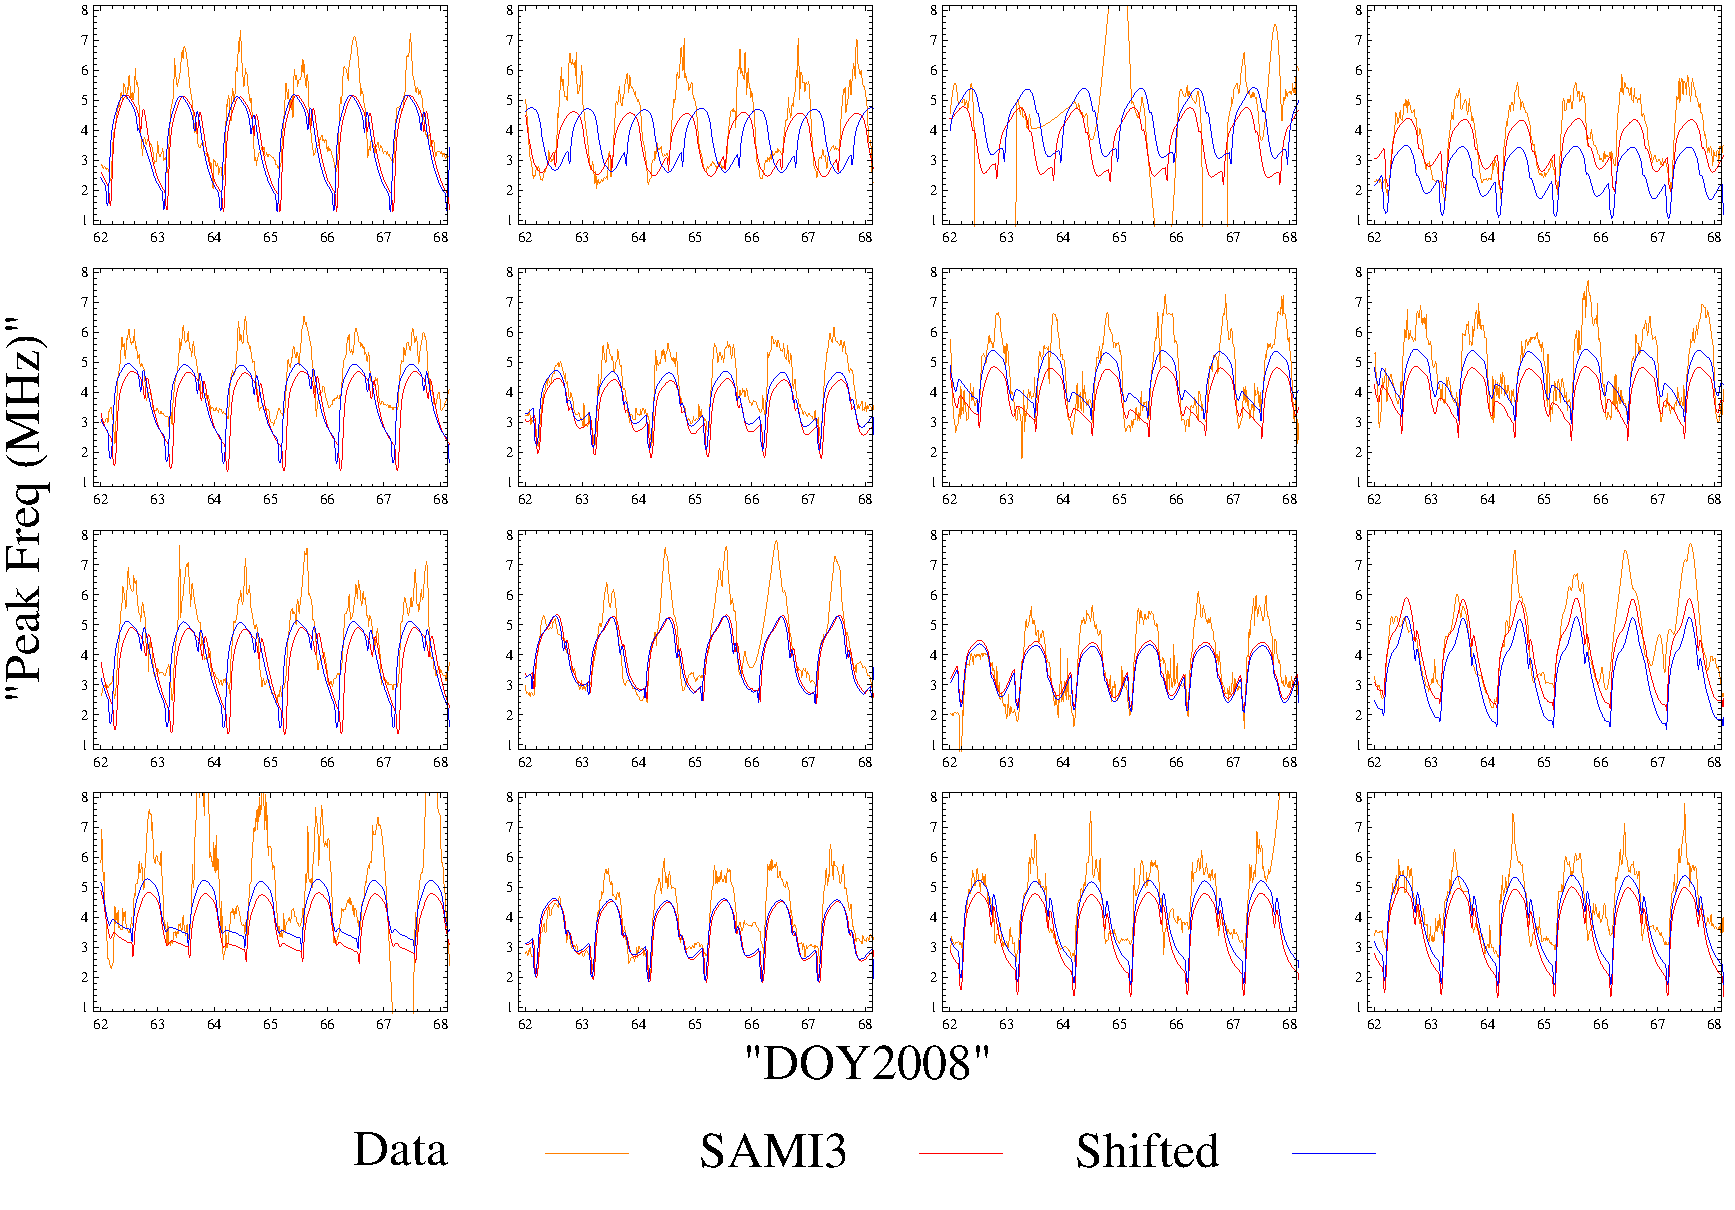
\includegraphics[width=\textwidth]{fs}
    \clearpage
  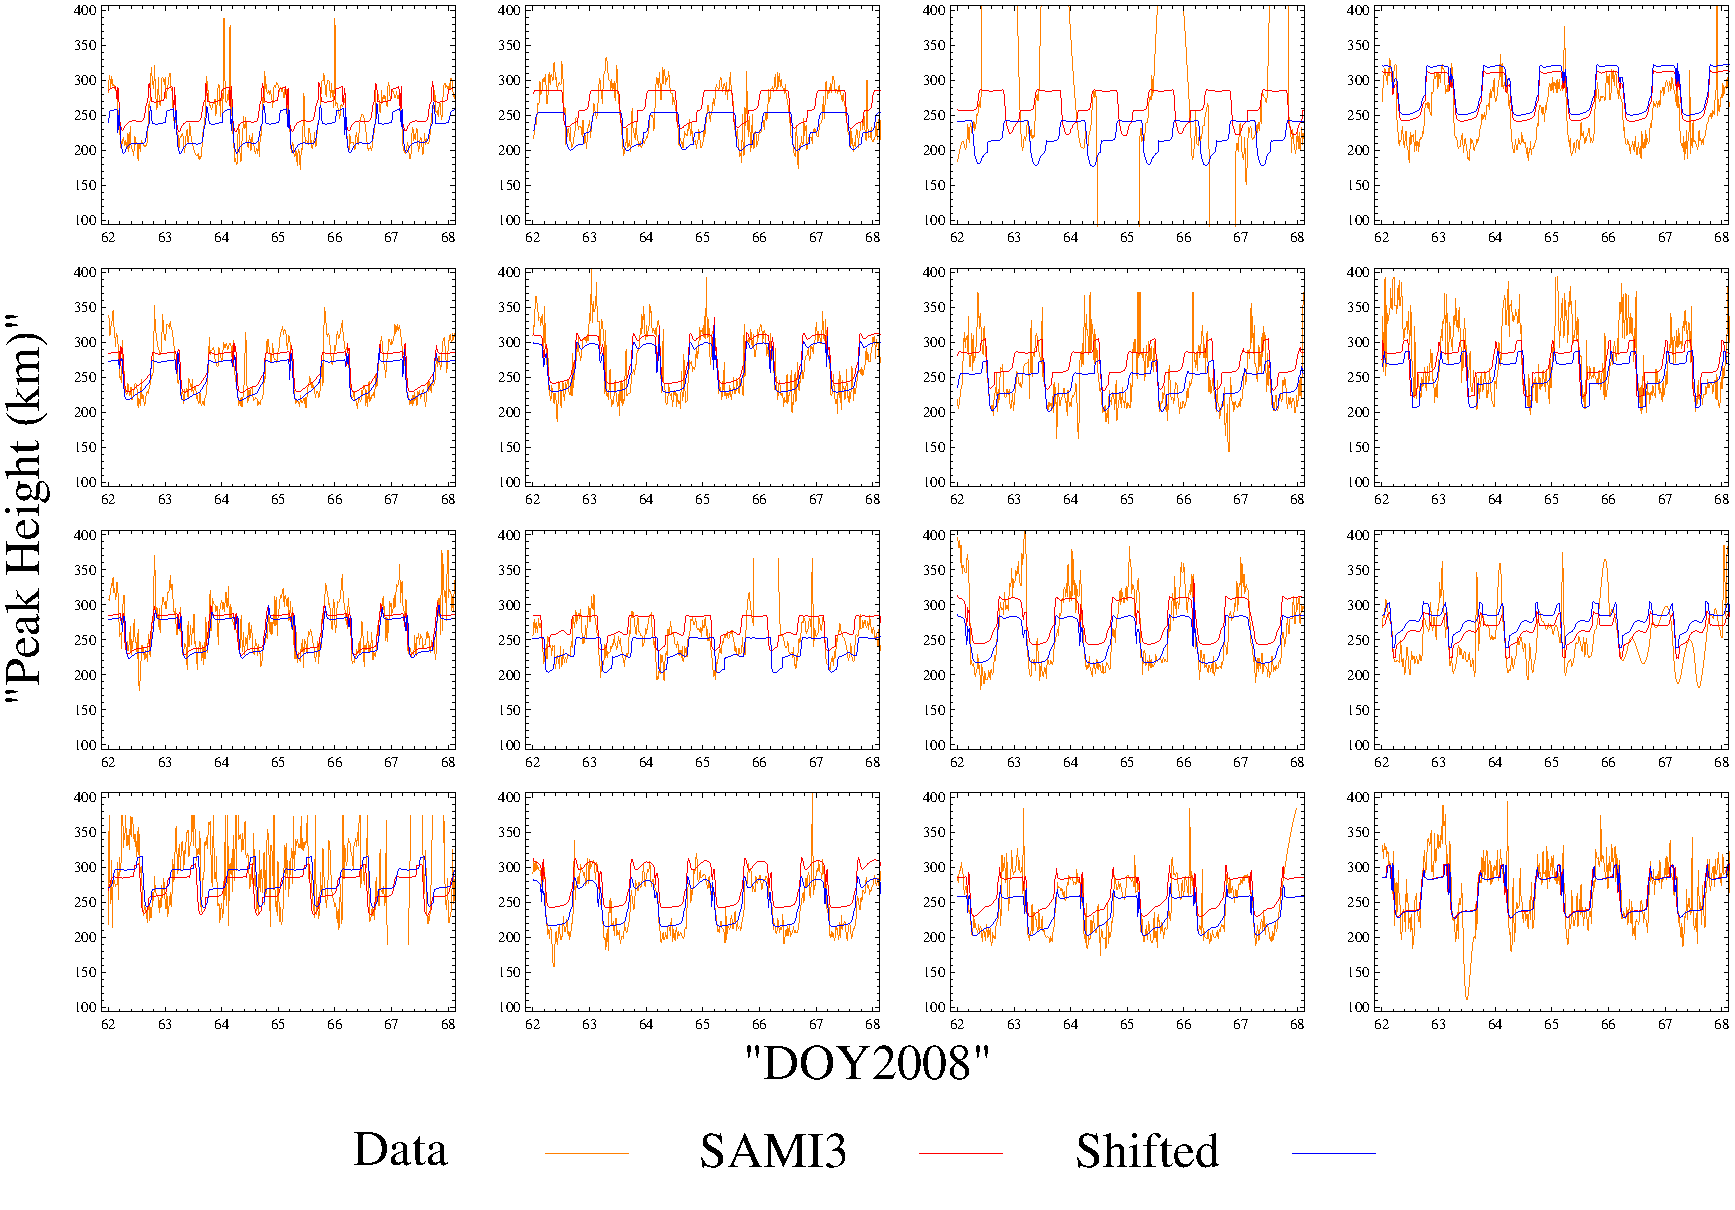
\includegraphics[width=\textwidth]{hs}

Also note that the total electron content (vertically integrated electron density) from SAMI3 is consistently higher than that of the actual ionosphere in 2008. This increased TEC and decreased electron density indicates a slab thickness that is too much. 
  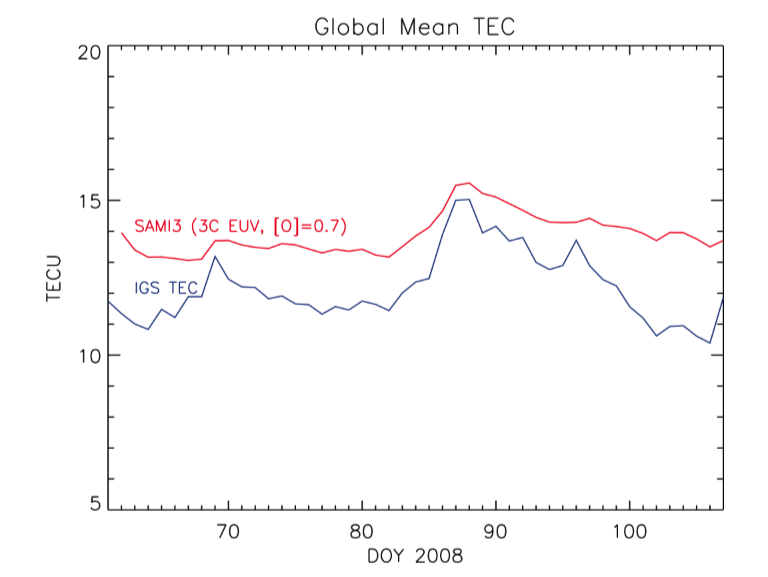
\includegraphics[width=.5\textwidth]{tec}
    \clearpage
    \clearpage
    These are the differences in frequency broken down by day. Again, a negative number indicates that SAMI is too low. 
  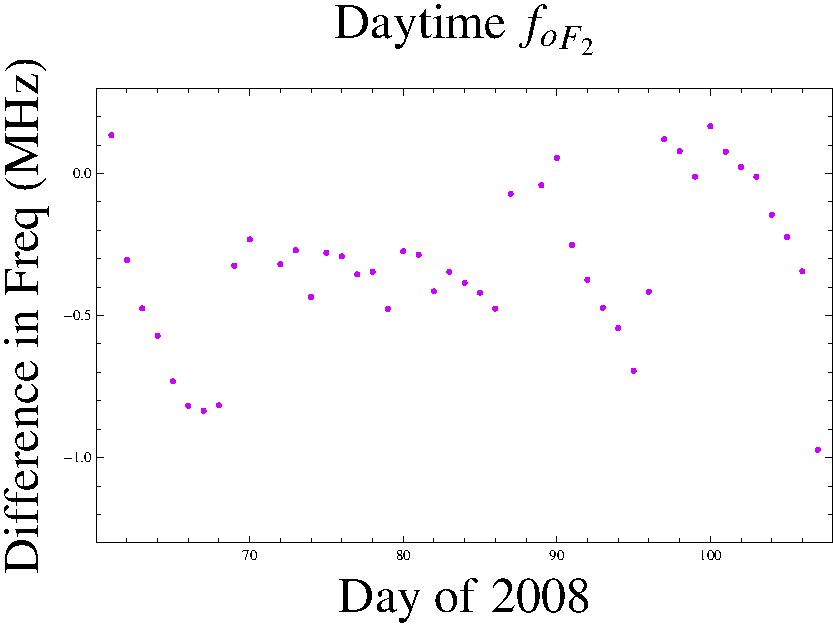
\includegraphics[width=.75\textwidth]{dayf}
  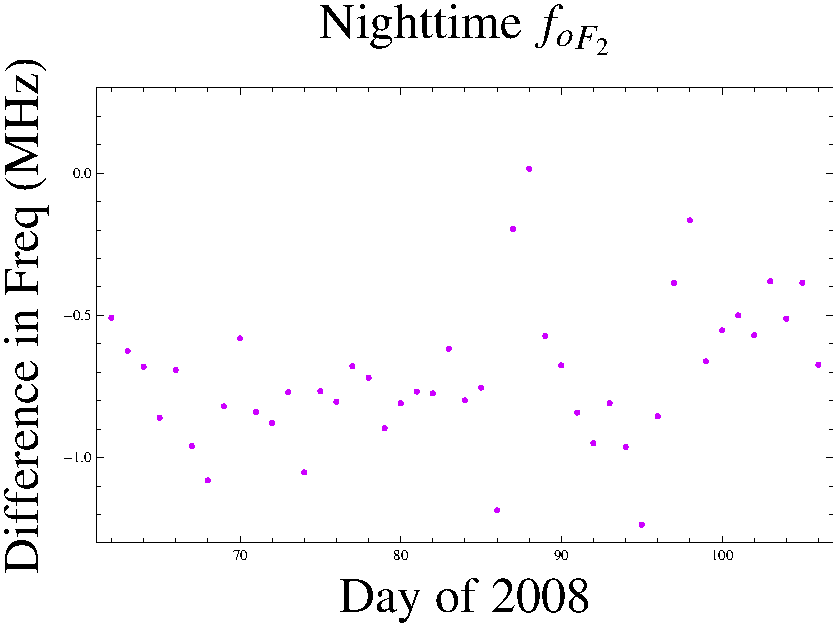
\includegraphics[width=.75\textwidth]{nightf}
    \clearpage
  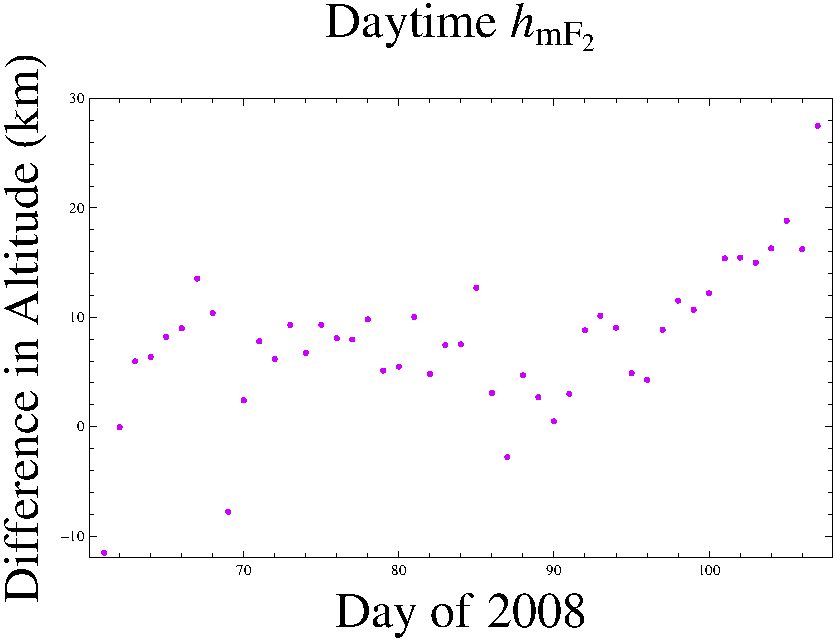
\includegraphics[width=.75\textwidth]{dayh}
  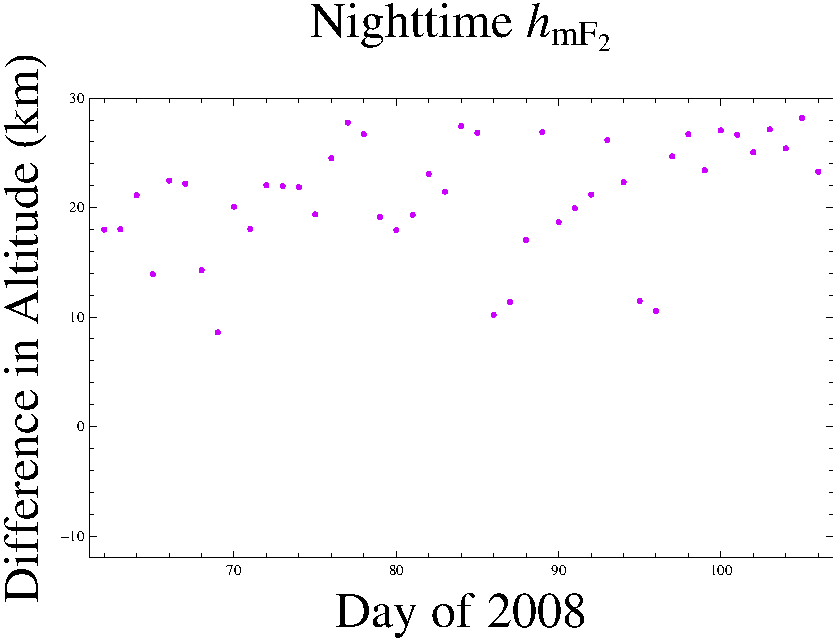
\includegraphics[width=.75\textwidth]{nighth}
    \clearpage

    \subsection{Modeling Experiments with SAMI2 {Effect of $T_{exo}$ and $\left[O\right]$}}
    Now, it is left to determine whether this is a problem with the physics in SAMI or the atmospheric conditions that are used as inputs to SAMI. Since SAMI3 is a large model, and it would take a significant amount of resources to test the behavior with various input conditions, this testing was done with SAMI2. The effect of [O] and scaling down the exospheric temperature was observed.

    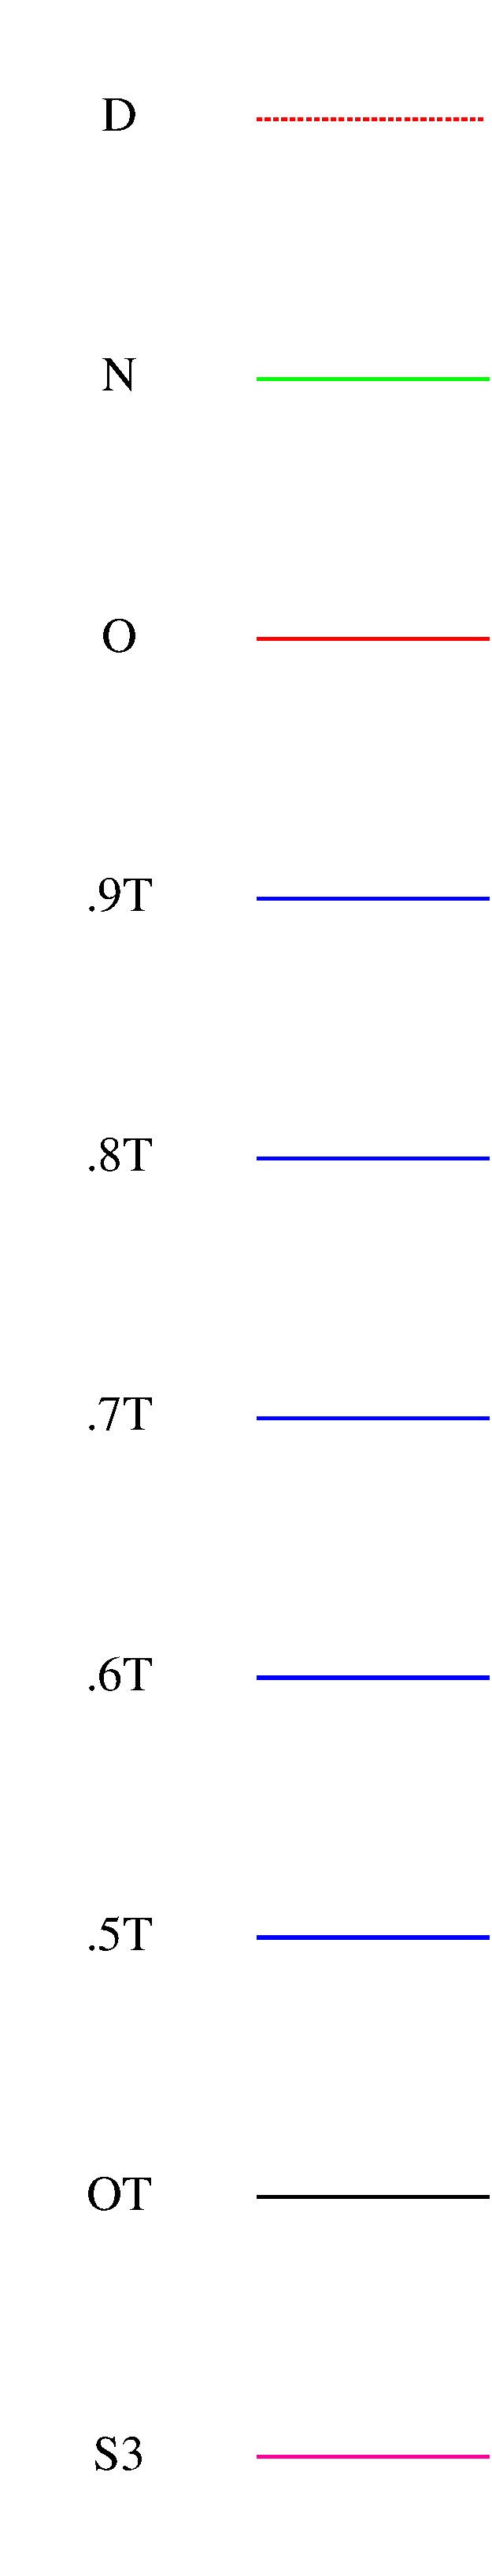
\includegraphics[height=4in]{legend}
    \includegraphics[height=4in]{fo}
    \clearpage

    The same breakdown for heights shows that it's off during specific points of the day  \\
    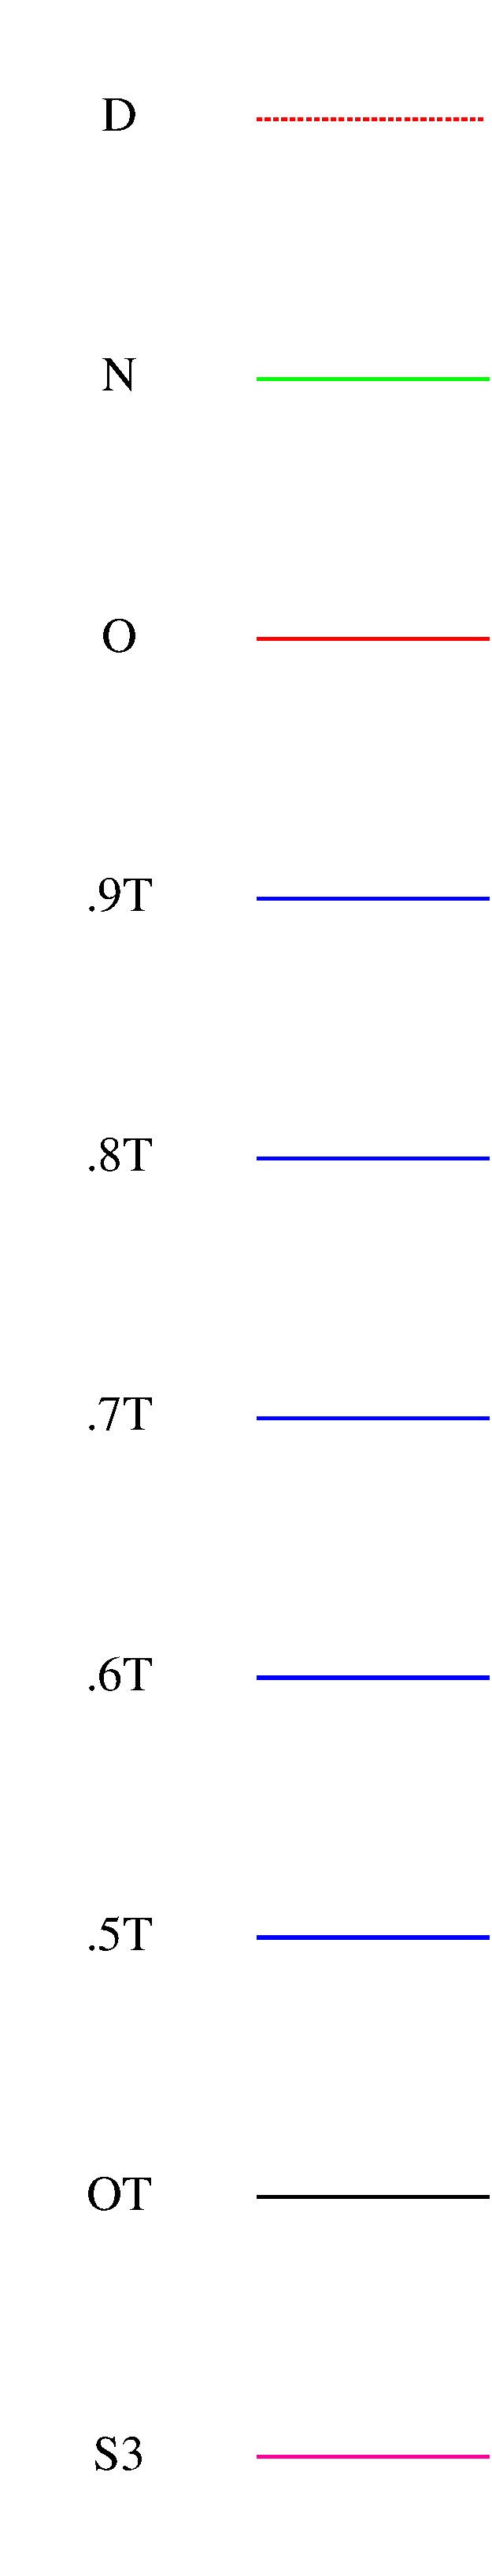
\includegraphics[height=4in]{legend}
    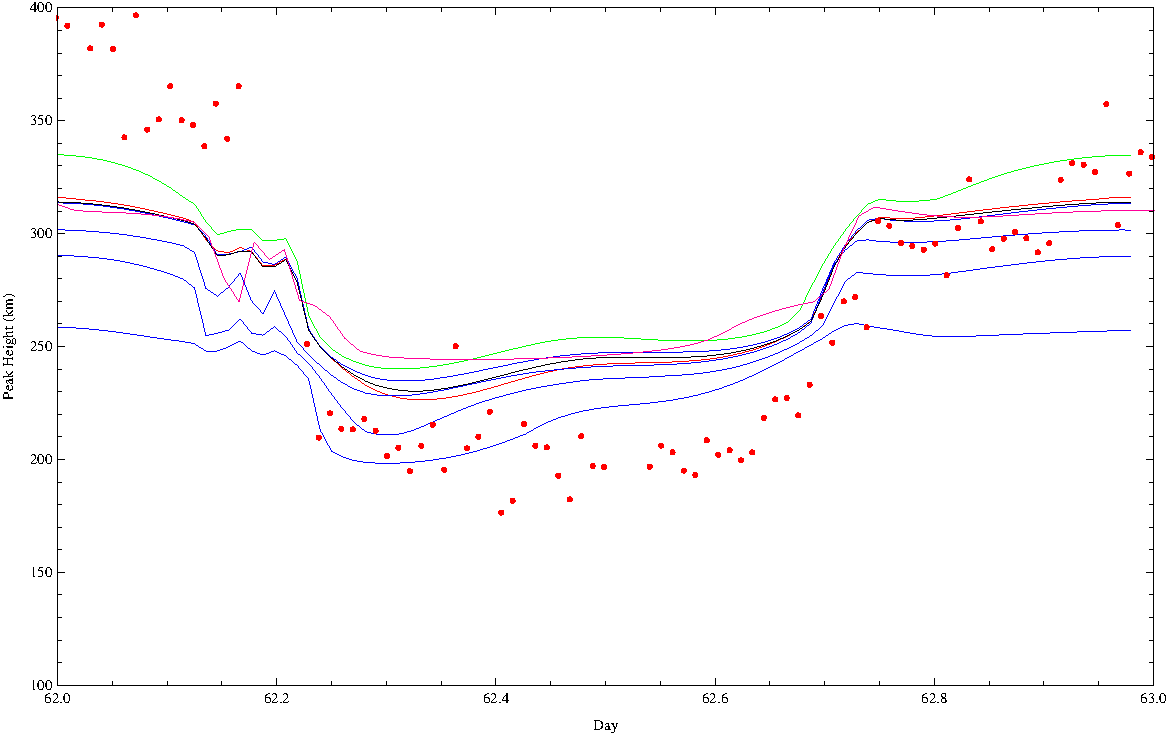
\includegraphics[height=4in]{hm}
    \clearpage


\section{Conclusion}
\IEEEPARstart T{he} output of SAMI3 was compared to ionosonde data on a global scale. As a first step, this paper describes comparisons made against measurements during the Whole Heliospheric Interval, a solar quiet time with historically low activity during the most recent solar minimum during the last solar cycle.  This reduces the dynamic inputs into the model, and takes out the most complicated part of modelling the ionosphere. 
  A systematic difference between the ionosonde data and the SAMI3 model was found at mid-latitude stations. During the daytime, SAMI3 has $F_2$ peak densities too low and $F_2$ peak slightly high, increasing towards the end of the interval.
  During the nighttime, the $F_2$  peak density is still consistently too low and the $F_2$ peak height is too high.
         Globally SAMI3 has higher TEC than GPS data, In spite of $f_oF_2$ (and $n_mF_2$) being systematically low.
         SAMI3 sometimes give unrealistic slab thickness 
   SAMI2 runs adjusting MSIS atmospheric parameters (Temperature and Density) were tested.
        Uncertainties in 2008 Solar Minimum Atmosphere do not fully explain systematic differences.
	Reduced Atmospheric Temperature was found, so MSIS density and temperature were adjusted to match Solar Minimum 2008 measurements
        Height differences were likely due to drifts and winds.
	  
	In the future, for further research, it is advisable to try adjusting $\vec E\times\vec B$ drifts to correct heights.
	    Drifts are expected to be smaller during 2008 Solar Minimum.
        Furthermore, it would be helpful to look at recombination rates at high altitudes.
	   At high altitudes, the recombination rate is proportional to [NH+][Ne]
	   The ionosphere transitions to being H+ dominated at lower altitudes during Solar Minimum, which would require further testing to determine if it was found correctly by the input models. The Mathematica code used for the analysis can be found at \texttt{\url{http://github.com/atondwal/sami_analysis}} .
\section{Acknowledgements}
 The author thanks his mentor Carl Siefring, and Paul Bernhardt and Jonathan Krall for their guidance.
\nocite{*}
\bibliographystyle{IEEEtran}
\bibliography{IEEEabrv,bib}
\end{document}
